\label{chap:intro}



\begin{marginfigure}
  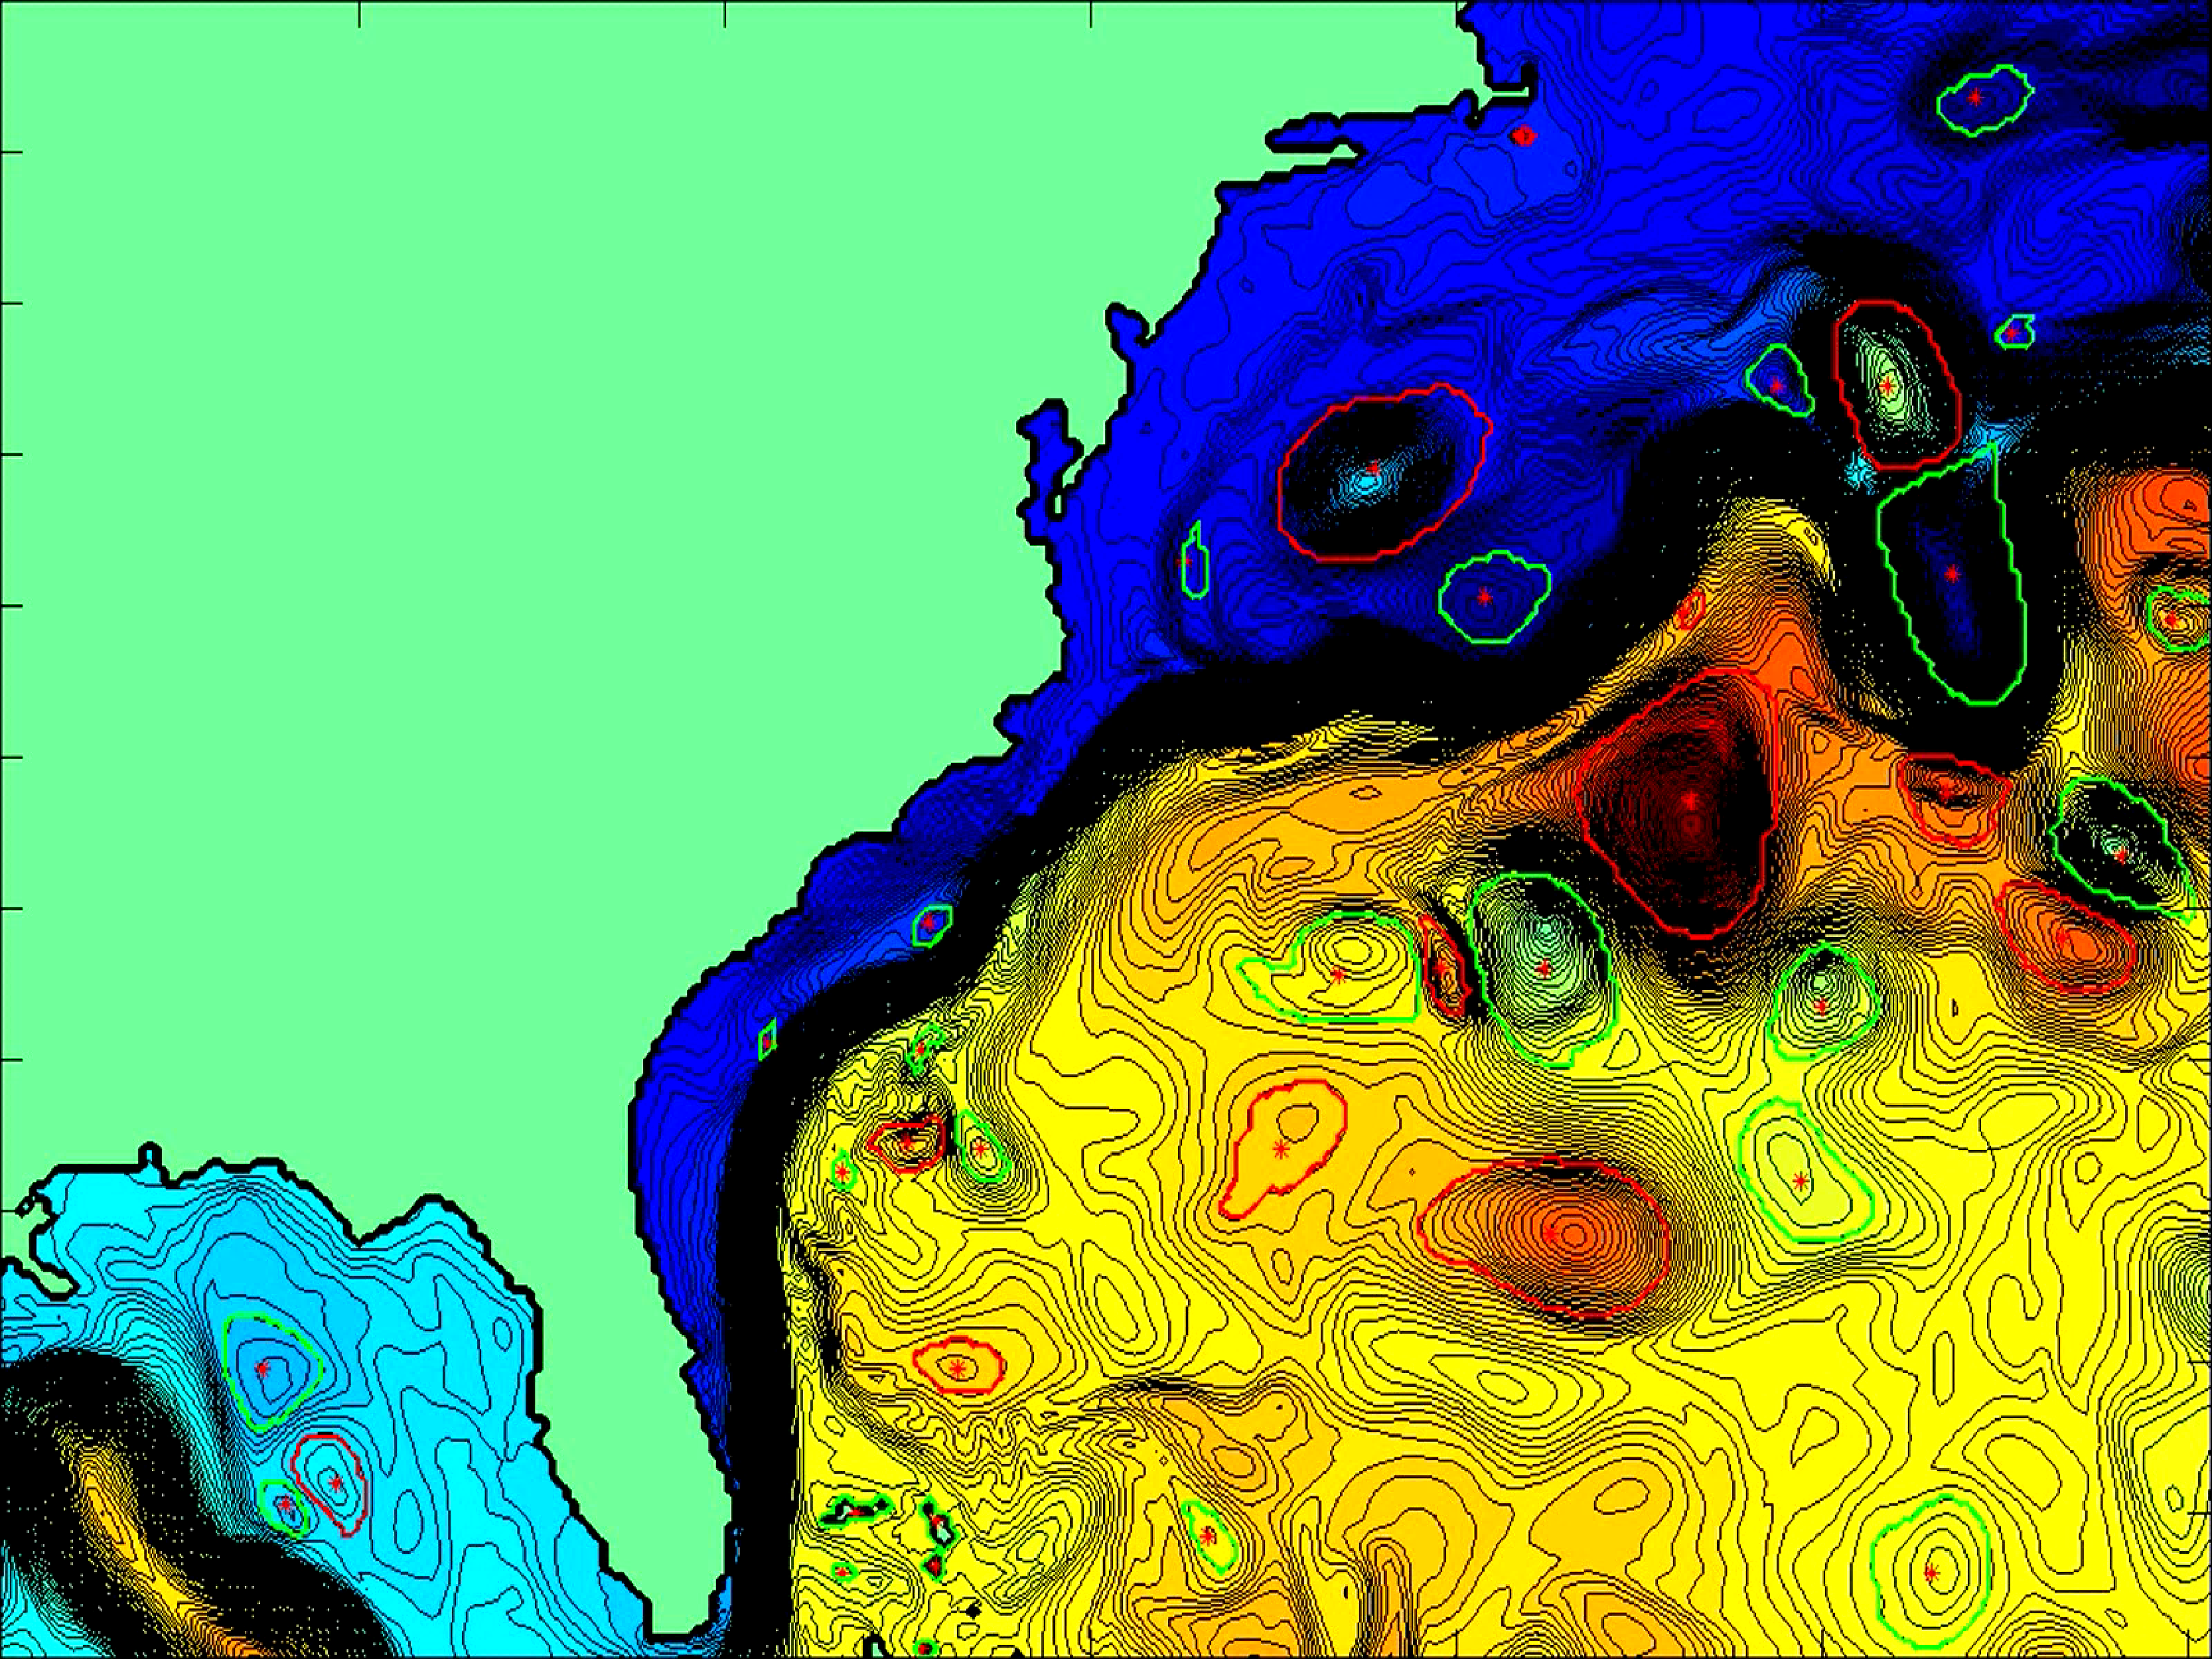
\includegraphics[]{GS.pdf}
\caption{Animation snapshot of early test run. Shown is SSH with detected eddies indicated.}
\end{marginfigure}


\paragraph{This}chapter discusses the theory of meso-scale turbulence and parametrizations thereof.
Geostrophic turbulence is typically characterized by rather stable, circular, coherent pressure anomalies, that rotate fluid around in a vortex in
quasi-geostrophic equilibrium. These entities can persist for long periods of time in which they often travel distances on the order of hundreds of kilometers
zonally. The fact that baroclinic instability forms these vortices instead of leading to a cascade to ever smaller scales ,as would be expected from chaotic
turbulence, is a direct consequence of the inverse energy cascade of 2-dimensional motion. For a discussion of this phenomenon see appendix
\ref{chap:turbu_categories}. The atmospheric analog are storms and high-pressure systems, yet with much less difference between high- and low-pressure systems due to
a smaller centrifugal force \ie smaller Rossby number. These quasi-geostrophic, meso-scale vortices, from here on called eddies \footnote{For a discussion of
the different types of vortices in the ocean see appendix \ref{chap:eddy_cat}}, are immediately visible on
SSH maps. Yet, it is difficult to physically \emph{define} an eddy in terms of oceanographic variables. The transition from meandering jets or other undeveloped
baroclinic turbulence is not very sharp. Eddies also sometimes merge or split or collectively form rifts and valleys in SSH. detecting them on one snapshot
automatically via an algorithm is therefore not trivial. Further problems arise when the algorithm is also supposed to track them. Their shear abundance at any
given time inevitably creates ambiguities between time steps. It is therefore necessary to set up a clear, unambiguous, sufficient (in the mathematical sense)
definition.\\

\subsection{Detection methods} \label{subsec:detectmethods}
\begin{itemize}
	\item
	One way to find an eddy in SSH-data is to simply scan for closed contours at different values for $\vec{z}$ and then subject found entity to a series of necessary tests. Only if all criteria are met is an eddy found. This method was first used by \citet{Chelton2011} and turned out to be the simplest yet most effective method, at least for satellite SSH data. Therefore, as a starting point, this method will be adopted and should also serve as a general definition of what will be referred to as an \textit{eddy} hereafter\footnote{The vortices will have names deviant from \textit{eddy} where these criteria are altered.}.\\
	\citeauthor{Chelton2011} set the following threshold criteria for his algorithm:
\begin{enumerate}
\item
The SSH values of all of the pixels are above (below) a given SSH threshold for anticyclonic (cyclonic) eddies.
\item
There are at least \textit{[threshold]} pixels and fewer than \textit{[threshold]} pixels comprising the connected region.
\item
There is at least one local maximum (minimum) of SSH for anticyclonic (cyclonic) eddies.
\item
 The amplitude of the eddy is at least \textit{[threshold]}.
\item
The distance between any pair of points within the connected region must be less than \textit{[threshold]}.
\end{enumerate}

\item
Another frequently used method do define an eddy makes use of the strain tensor $\ten{T}$\derref{der:okubo}. The trace of the strain tensor squared includes
valuable information about the dynamics of the velocity field. Namely
%%....................................................................
\begin{equation}\begin{split}
	2\mathrm{O_w}=\tr{\ten{T}^2}
	=
	divergence^2
	+ stretching^2
	+ shear^2
	 - vorticity^2 \\
\end{split}\end{equation}
%%....................................................................
which reduces to $\mathrm{O_w}= \left(\partial_x u\right)^2+2 \partial_y u \partial_x v$ in 2 dimensions. This is called the
Okubo\footnote{\citet{Okubo1970}}-Weiss-Parameter. It is a useful tool to determine whether the field has parabolic, vorticity dominated character, or whether
deformation dominates giving hyperbolic character. An area of large negative values indicates high enstrophy density compared to gradients of kinetic energy,
thus indicating little friction paired with high momentum \ie a coherent, angular-momentum-conserving entity. Positive values on the other hand indicate
incoherent deformation.\\ As genius as this parameter seems, it turns out that using it to identify eddies is often not the best solution.
\citeauthor{Chelton2011} names 3 major drawbacks:
\begin{itemize}
	\item
	\textit{ No single threshold value for $\mathrm{O_W}$ is optimal for the entire World Ocean. Setting the threshold too high can result in failure to identify small eddies, while a threshold that is too low can lead to a definition of eddies with unrealistically large areas that may encompass multiple vortices, sometimes with opposite polarities. }
	\item
	$\mathrm{O_W}$ is highly susceptible to noise in the SSH field. Especially when velocities are calculated from geostrophy, the sea surface has effectively
been differentiated twice and then squared, exacerbating small incontinuities in the data.
	\item
	\textit{The third problem with the W-based method is that the interiors of eddies defined by closed contours of W do not generally coincide with closed contours of SSH. The misregistration of the two fields is often quite substantial. }
\end{itemize}
It is hence only logical to scan for closed contours of SSH directly (as was done so by \citeauthor{Chelton2011}).
\end{itemize}
